\documentclass{article}

\usepackage[french]{babel}
\usepackage[utf8]{inputenc}
\usepackage[T1]{fontenc} 
\usepackage{graphicx}
\usepackage{mathtools, bm}
\usepackage{amssymb, bm}
%%%%%%%%%%%%%%%% Lengths %%%%%%%%%%%%%%%%
\setlength{\textwidth}{15.5cm}
\setlength{\evensidemargin}{0.5cm}
\setlength{\oddsidemargin}{0.5cm}

%%%%%%%%%%%%%%%% Variables %%%%%%%%%%%%%%%%
\def\projet{1}
\def\titre{Méthodes de calcul numérique \\ Limites de la machine}
\def\groupe{3}
\def\equipe{2}
\def\responsible{Imad BOUDROUA}
\def\secretary{Mohamed Faycal BOULLIT}
\def\others{Theo LELASSEUX,\\ Deborah PEREIRA,\\ Mohammed BOUDALI}

\begin{document}

%%%%%%%%%%%%%%%% Header %%%%%%%%%%%%%%%%
\noindent\begin{minipage}{0.98\textwidth}
  \vskip 0mm
  \noindent
  { \begin{tabular}{p{7.5cm}}
      {\bfseries \sffamily
      Projet \projet} \\ 
      \itshape \titre
    \end{tabular}}
  \hfill 
  \fbox{\begin{tabular}{l}
      {~\hfill \bfseries \sffamily Groupe \groupe\ - Equipe \equipe
        \hfill~} \\[2mm] 
      Responsable : \responsible \\
      Secrétaire : \secretary \\
      Codeurs : \others
    \end{tabular}}
  \vskip 4mm ~

  ~~~\parbox{0.95\textwidth}{\small \textit{Résumé~:} \sffamily
\indent Ce projet a pour but d'évaluer les problèmes qui peuvent apparaître lors de l'utilisation d'opérations élémentaires et d'algorithmes sur des flottants. Il traite dans un premier temps de la précision insuffisante des opérations élémentaires dans des cas particuliers, et dans un second temps, d'algorithmes utilisés dans des conditions de calcul en basse précision, comme l'algorithme de CORDIC utilisé dans les calculatrices. }
  \vskip 1mm ~
\end{minipage}

%%%%%%%%%%%%%%%% Main part %%%%%%%%%%%%%%%%
\section{Représentation des nombres en machine}
\
\indent Cette partie consiste à aborder certains exemples et appliquer les notions vues en cours pour pouvoir déterminer les différents types d'erreur.
En effet, chaque flottant sur la machine est approximé, et après chaque opération élémentaire, on a une erreur induite de calcul, ce qui est mis en évidence dans cette partie à travers l'implémentation de la fonction \textbf{rp(x,p)}. %sur le graphe --- .
%\subsection{Algorithmes implémentés}
\subsection{Représentation décimale réduite rp(x,p)}
\indent Pour l'implémentation de l'algorithme de calcul de la représentation décimale réduite, nous avons utilisé la fonction \textbf{round(n,p)} qui  arrondi avec un nombre flottant n à p décimales. Pour "tronquer" \texttt{x} à l'aide de \texttt{round(x,m)}, il faut donc connaître l'exposant k en notation scientifique de \texttt{x}. L'algorithme traite deux cas: 
\begin{itemize}
\item $x < -1$ ou $x > 1$: diviser par 10 une variable temporaire t tant que  $x*t>=10$ ou $x*t<=-10$ en incrémentant le compteur k. 
\item $-1\leq x \leq1$: Tant que $-1\leq x*t \leq1$ t est multipliée par 10 à chaque fois en incrémentant k.
\end{itemize}

\indent Dans les deux cas on cherche donc à représenter x par sa notation scientifique : $x=m*10^k$ afin de pouvoir appliquer round sur m et obtenir ainsi la représentation en décimale réduite de x.
\subsection{Opérations usuelles}
Dans cette section nous allons effectuer les opérations usuelles addition et multiplication en représentation décimale réduite.
\subsubsection{Addition et multiplication}
L'algorithme adopté dans ces opérations est le suivant:
\begin{enumerate}
    \item Les représentations décimales réduites de x et y sont récupérées.
    \item L'addition ou la multiplication est effectuée.
    \item La représentation décimale réduite du résultat est récupérée.
\end{enumerate}
\subsubsection{Erreurs relatives}

On calcule l'erreur relative de l'addition et la multiplication sur x et y en représentation décimale réduite d'après la formule donnée dans le sujet. On obtient alors le graphique suivant :
\begin{figure}[h]
    \centering
    \centerline{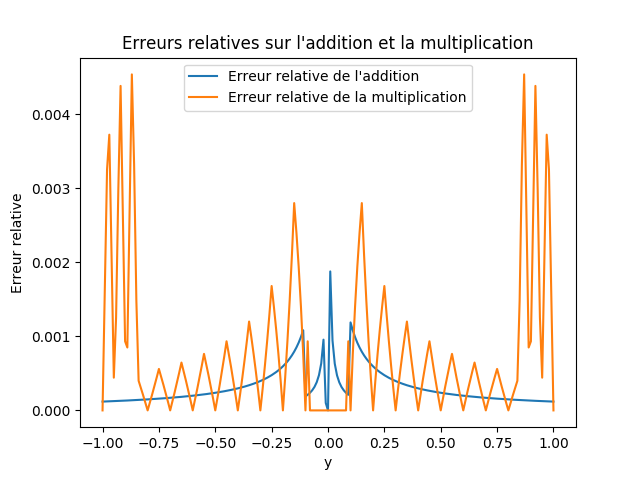
\includegraphics[width=8cm]{Figure_1.png}}
    \caption{Erreur relative sur l'addition et la multiplication de x et y avec x=0.000119}
    \label{ERREUR}
\end{figure}

\subsubsection{Calcul de log(2)}

Pour calculer log(2) on calcule la somme de de $\frac{(-1)^{i+1}}{i}$ avec i allant de 1 à 100. Pour cela on utilise une boucle qui à chaque tour ajoute à notre somme s le terme $\frac{(-1)^{i+1}}{i}$. Une fois que i=100, on calcule la représentation décimale réduite à p décimales de cette valeur et on calcule l'erreur relative avec la valeur calculée par la fonction log de numpy. On constate que quelque soit p, l'erreur relative est nulle. L'algorithme que nous avons trouvé a donc la même précision que celui de numpy.

\section{Algorithmes CORDIC}
\indent Dans cette partie, nous allons nous intéressé à l'implémentation de quelques fonctions en utilisant les algorithmes \textbf{CORDIC} utilisés dans des conditions où on ne possède pas de ressources importantes(mémoire, puissance de calcul) pour effectuer des calculs. C'est le cas pour les calculatrices de poche.

\subsection{Représentation des nombres sur une calculatrice}
\
\indent Dans une calculatrice typique un nombre 'flottant' occupe 8 octets de mémoire et se décompose en :
\par     - une mantisse constituée de 13 chiffres codés indépendamment sur 4 chiffres binaires (on parle de Binaire Code Decimal ou BCD) 
\par     - un exposant (puissance de 10) éventuellement signé
\par     - le signe du nombre (et de l'exposant s'il n'est pas signé)

Cette représentation permet de représenter un très large intervalle de nombres réelles. Cependant, cette représentation occupe un peu plus de place, car il est nécessaire de coder la position de la virgule. De plus, pour de grand nombre on perd en précision, les chiffres de poids faible n'étant alors plus représentés. 
  
\subsection{Fonctions trigonométriques et exponentielles}
\
\indent Le principe des algorithmes \textbf{CORDIC} est d'effectuer une série de transformations simples (addition/soustraction et décalage) réduisant la valeur de x à une valeur très faible en même temps qu'en élaborant le résultat. Chacune de ces transformations nécessite une valeur pré-calculée de f (ou de son inverse). Le résultat est obtenu par une simple interpolation linéaire (ou un développement en série si davantage de chiffres sont requis).

Tout d'abord, il est nécessaire de ramener la valeur à calculer ,soit x, dans un intervalle où on peut appliquer l'algorithme, tout en effectuant des transformations simples (addition/soustraction et décalage)

Pour l'exponentielle par exemple, il faut ramener la valeur à calculer x dans l'intervalle $ [0,ln(10)[ $ en trouvant un entier n réalisant : $ exp(x)= exp(x-n*ln(10))*10^n $

Et donc il suffit de calculer $exp(x-n*ln(10))$ par l'algorithme de \textbf{CORDIC} puis multiplier par $ 10^n $

Cette technique est efficace lorsqu’elle est ramenée à une calculatrice pour les raisons suivantes :
\par - L'utilisation exclusive des deux opérations : addition et soustraction (opérations de faible coût), ce qui permet de minimiser le temps de calcul.
\par - L'utilisation de valeurs pré-calculées : en effet, la recherche d'une valeur dans un tableau prend moins de temps que de réaliser le calcul, généralement, lourd de cette valeur.

Pour tester les fonctions implémenter on a tracé les graphes dans la figure \ref{CORDIC} qui correspondent à l'erreur relative entre les valeurs calculées par l'algorithme \textbf{CORDIC} et ceux des fonctions de la bibliothèque MATH en python. Les graphiques correspondent successivement à l'erreur relative de la fonction logarithme, exponentielle, arctangente et tangente.

\begin{figure}[h]
    \centering
    \centerline{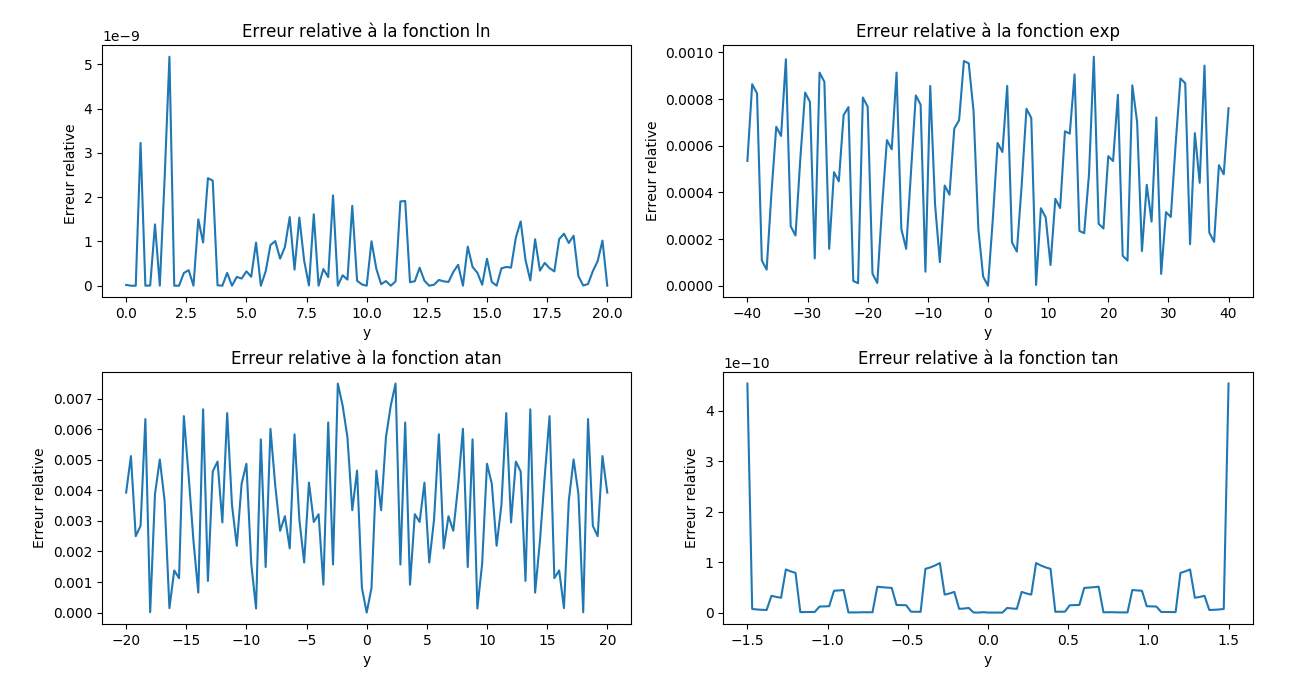
\includegraphics[width=18cm]{Figure_2.png}}
    \caption{Erreurs relatives pour les fonctions implémentées par les algorithmes CORDIC}
    \label{CORDIC}
\end{figure}
On remarque que pour la fonction logarithme népérien pour $x\in[0,20]$ l'erreur relative maximale est de $5*10^{-9}\%$.
Pour la fonction exponentielle  pour $x\in[-40,40]$ l'erreur relative maximale est de 0,001\%.
Pour la fonction arctangente pour $x\in[-20,20]$ l'erreur relative maximale est de 0,008\%.
Pour ces trois fonctions, aucun comportement particulier de l'erreur relative n'est notable. 
Pour la fonction tangente pour $x\in[-1.5,1.5]$ l'erreur relative maximale est de $4,6*10^{-10}\%$. On constate que plus x est proche de la valeur $\frac{\pi}{2}$ ou $-\frac{\pi}{2}$, plus l'erreur relative est importante. Cela est dû au fait qu'on cherche à calculer une valeur très grande, la fonction tangente tendant vers l'infini. 
\\
\\
\\
\subsection{Problèmes soulevés dans \textit{Numerical Recipes in C}}

\subsubsection{Arithmétique sur les complexes}
\
\indent Afin d'évaluer une multiplication entre deux complexes, il est possible d'utiliser l'expression suivante :
\begin{equation}
    (a + ib)(c + id) = (ac - bd) + i(bc + ad)
\end{equation}
\indent On utilise alors 4 multiplications, 1 addition et 1 soustraction.
Il est possible d'utiliser une autre expression :
\begin{equation}
    (a + ib)(c + id) = (ac - bd) + i[(a + b)(c + d) - ac - bd]
\end{equation}
\indent On utilise cette fois 3 multiplications, 2 additions et 3 soustractions. On utilise plus d'opérations au total, mais 1 multiplication de moins ce qui est rentable au vu du coût d'une multiplication par rapport à une addition ou soustraction.
\medbreak
Dans le cas du calcul du module d'un complexe, il est fortement déconseillé d'utiliser l'expression classique du module :
\begin{equation}
    |a + ib| = \sqrt{a^2 + b^2}
\end{equation}
\indent En effet, si a ou b est aussi grand que la racine carrée du plus grand nombre représentable, un overflow a lieu.
Il est donc préférable d'utiliser l'expression suivante :
\begin{equation}
    |a + ib| = |a|*\sqrt{1 + (\frac{b}{a})^2} si |a| >= |b|
\end{equation}
\begin{equation}
    |a + ib| = |b|*\sqrt{1 + (\frac{a}{b})^2} si |a| < |b|
\end{equation}
\subsubsection{Fractions continues}
\
\indent Les fractions continues sont un outil puissant pour évaluer des fonctions. Une fraction continue est une expression de la forme :
\begin{equation} \label{eq1}
b_0+\frac{a_1}{b_1+\frac{a_2}{b_2+\frac{a_3}{b_3+\frac{a_4}{..}}}}
\end{equation} comportant un nombre fini ou infini d'étages.
\medbreak
Le problème posé par les fractions continues est le suivant : \textbf{comment savoir jusqu'où aller lorsqu'on évalue une fraction continue ?}
\medbreak
Contrairement à une série, on ne peut pas simplement évaluer l'équation de gauche à droite jusqu'à ce que le terme suivant à ajouter n'apporte qu'un faible changement. Écrite sous la forme de (\ref{eq1}), la seule façon d'évaluer la fraction continue est de droite à gauche, ce qui nous obligerait à choisir aveuglément un point de départ. Pour éviter cela, il faut utiliser un résultat qui relie les fractions continues aux approximations rationnelles, et qui donne un moyen d'évaluer notre fraction continue de gauche à droite. Notons $f_n$ le résultat de l'évaluation de (\ref{eq1}) au rang n :
\begin{equation} \label{eq2}
    f_n=\frac{A_n}{B_n}
\end{equation}
Avec :
\begin{equation}
    A_{-1}=1,\ \ \ \ \ A_0=b_0,\ \ et \ \ \ A_j=b_jA_{j-1}+a_jA_{j-2}\ \ \ \ j=1,2,..,n
\end{equation}
\begin{equation}
    B_{-1}=0,\ \ \ \ \ B_0=1,\ \ et \ \ \  B_j=b_jB_{j-1}+a_jB_{j-2}\ \ \ \ j=1,2,..,n
\end{equation}

Notre fraction continue, ainsi écrite sous la forme (\ref{eq2}) peut être évaluée de gauche à droite comme pour une série.


\subsubsection{Evaluation de polynômes}
\
\indent Un polynôme de degré N peut être représenté par un tableau de coefficients tel que c[j] est le coefficient de $x^j$. 

Pour évaluer un polynôme de degré 5 on peut simplement calculer :
\begin{equation}
    P(x)=c[0]+c[1]*x+c[2]*x*x+c[3]*x*x*x+c[4]*x*x*x*x+c[5]*x*x*x*x*x
\end{equation}
\indent Cependant cette méthode d'évaluation n'est pas du tout optimale. En effet ici on a 15 multiplications et 5 additions. On préférera donc faire : 
\begin{equation}
    P(x)=c[0]+x*(c[1]+x*(c[2]+x*(c[3]+x*(c[4]+x*c[5])))
\end{equation}
\indent Ce qui nous permet de réduire le nombre de multiplication à 5, avec toujours 5 additions. Cette astuce qui n'est rien d'autre que de la factorisation nous permet d'évaluer un polynôme de degré N en N multiplications.
\end{document}
